\chapter{Implementace webové aplikace}
\label{chap:implementation}

Vytvořený nástroj je editor ve formě webové aplikace. Ke zformování byly použité výše popsané technologie Angular a Konva.js. 
Jedná se o tzv. \emph{single page application (SPA)}, kde veškerý obsah a funkcionalita se nachází pouze na straně klienta a neexistuje žádný
serverový backend. Stavový management je vyřešen pomocí sdílené služby, která uchovává potřebná data k vykreslování objektů na plátno.
Stavy jsou při každém potřebném překreslení aktualizovány. Díky tomuto lze celý projekt jednoduše uložit do souboru a kdykoli znovu načíst.
    
\section{Vykreslování plátna}
    O vykreslování se stará několik Angularových služeb dohromady. Důvod je ten, že k určitým objektům je nutno změnit způsob jakým jsou vytvořeny a vykresleny.
    Informace o tom co se má vykreslit jsou jim předávány přes komponenty, které mají služby v sobě injektované. Tyto komponenty reagují
    na jakékoli změny, které uživatel provede v uživatelském rozhraní a jsou ihned reflektovány na plátno.

\section{Práce s aplikací}
    Uživatelské rozhraní, vyobrazené na obrázku \ref{fig:ad-editor-ui}, se podobá wireframu a je vytvořeno tak, aby bylo pro uživatelé co nejpřívětivější a líbivé.
    Ukázku práce s aplikací a další ukázky UI se nachází v příloze této práce.
    \begin{figure}[h]
        \centering
        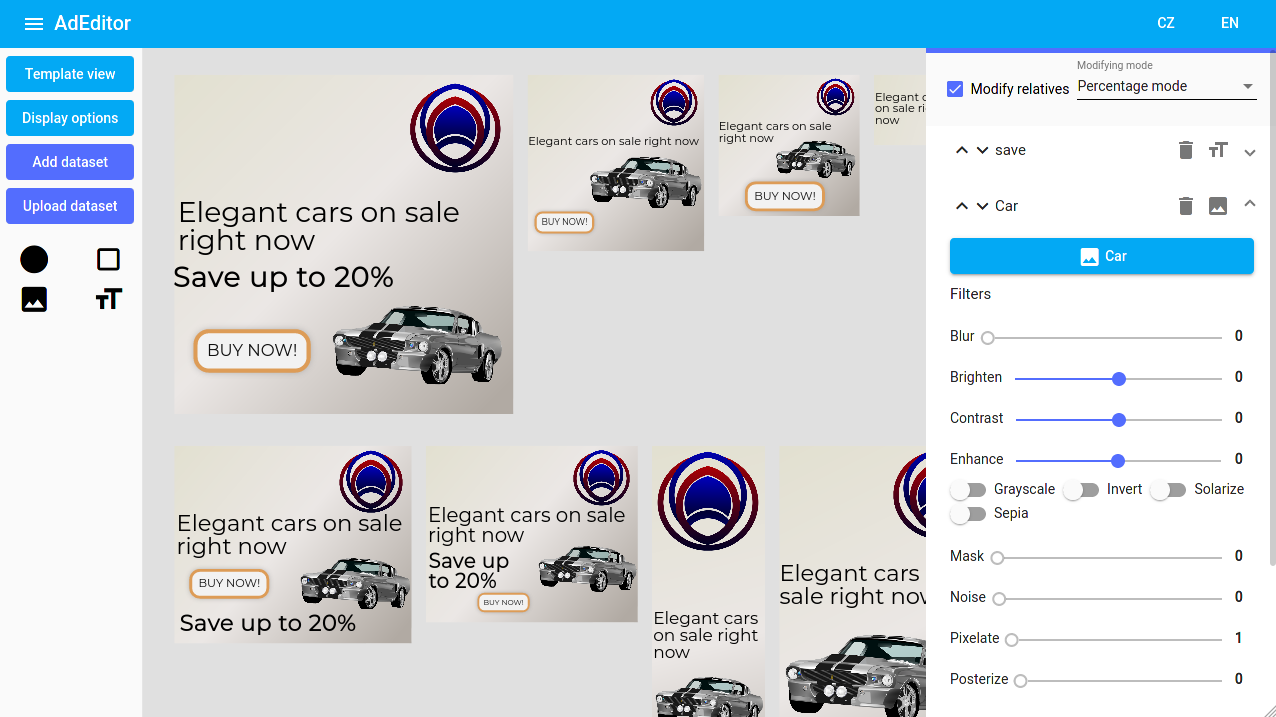
\includegraphics[width=1\textwidth]{Figures/ad-editor.png}
        \caption[UI webové aplikace]{Výsledné uživatelské rozhraní webové aplikace}
        \label{fig:ad-editor-ui}
    \end{figure}
    Při spuštění aplikace se uživateli zobrazí dialogové okno s výběrem velikostí bannerů. Po vybrání se náhledy bannerů vykreslí na plátno.
    První co uživatel upravuje je šablona, do které lze ihned umístit 4 základní prvky -- pozadí, logo, titulek a CTA.
    Při práci s prvky (jako je např. škálování a přetahování) na jednom banneru
    se tyto akce na daném prvku provádějí i na všech ostatní bannerech. Toto chování usnadňuje a urychluje celkovou tvorbu.
    Pro drobné úpravy si může uživatel tuto funkci vypnout.
    Dále je možno přidat na bannery více textů, obrázků, kruhů nebo čtverců. Dvojitým klikem na čtverec se z něj stane polygon, který lze libovolně upravovat
    přidáváním nebo odebíráním bodů. Pokud je potřeba, některé objekty zobrazovat pouze na některých bannerech, je toto nastavení taktéž umožněno.
    Nástroj pro všechny objekty poskytuje obvyklé možnosti úpravy.        

\section{Nahrávání datasetů}
    Všechny vykreslované objekty musí být unikátně pojmenované.
    Nahrávaný dataset musí být ve formátu CSV. Jako hlavička CSV souboru musí být uvedeny názvy objektů, které si uživatel přeje změnit, v tzv. \emph{slugu} (tzn. vše malými písmeny a mezery
    nahrazené pomlčkou). Měněné objekty, mohou být pouze texty nebo zdroje obrázků. Obrázky aplikace umožňuje načítat i ze vzdálených zdrojů skrz 
    URL adresu, ale vzdálený server musí povolit \emph{CORS}. Po úspěšném nahrání se do aplikace tyto datasety přidají a lze mezi nimi přepínat a každý
    individuálně dále upravovat.

\section{Export bannerů}
    Jakmile je uživatel s výsledkem spokojen, může bannery exportovat. Po zvolení exportu se zobrazí dialogové okno s nastavením exportu.
    Uživatel si může vybrat datasety k exportování, zda chce exportovat i šablonu, výstupní formát a případně poměr pixelů.
    Podporované výstupní formáty jsou JPEG a PNG. Pokud je zvolen JPEG, lze změnit i výslednou kvalitu.
    Dialog také zobrazuje největší odhadovanou velikost souboru, aby si uživatel nastavil vyhovující formát, případně kvalitu.
    Následně jsou vybrané datasety exportovány a staženy v ZIP archivu.




\endinput